% Created by tikzDevice version 0.12.3.1 on 2022-02-12 23:08:34
% !TEX encoding = UTF-8 Unicode
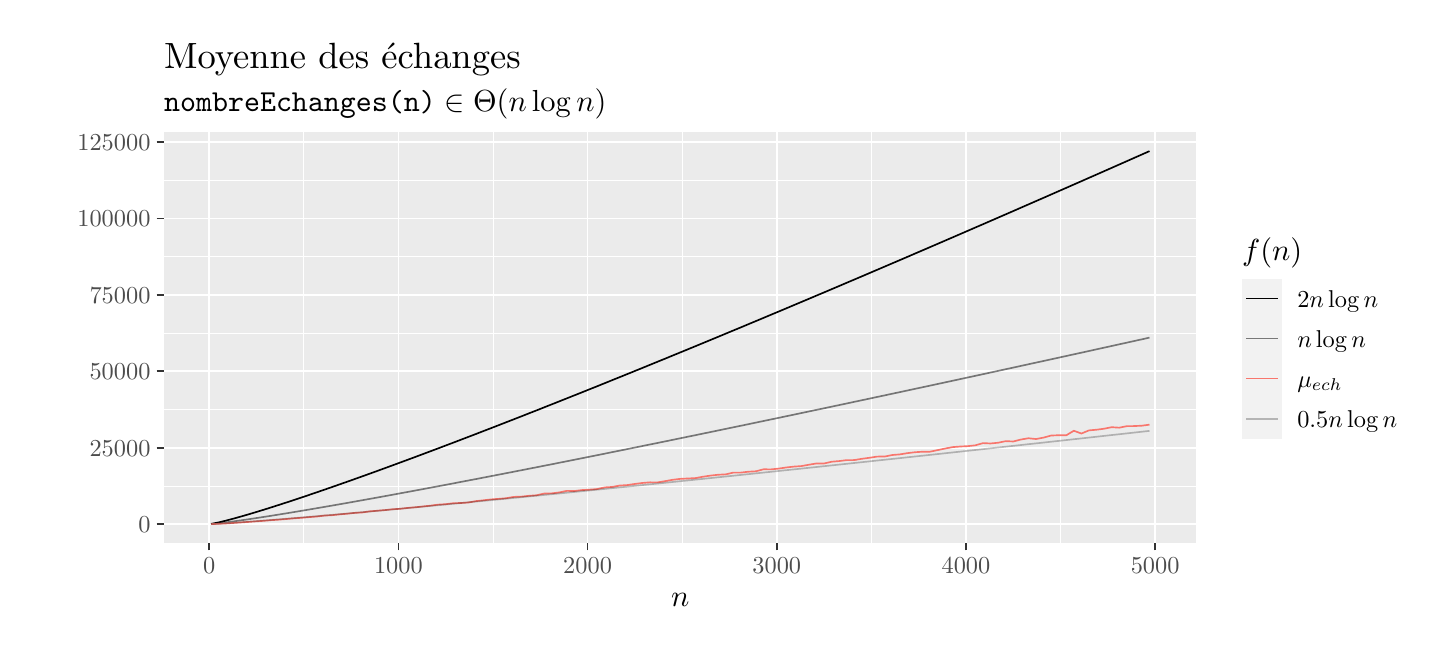
\begin{tikzpicture}[x=1pt,y=1pt]
\definecolor{fillColor}{RGB}{255,255,255}
\path[use as bounding box,fill=fillColor,fill opacity=0.00] (0,0) rectangle (505.89,216.81);
\begin{scope}
\path[clip] (  0.00,  0.00) rectangle (505.89,216.81);
\definecolor{drawColor}{RGB}{255,255,255}
\definecolor{fillColor}{RGB}{255,255,255}

\path[draw=drawColor,line width= 0.6pt,line join=round,line cap=round,fill=fillColor] (  0.00,  0.00) rectangle (505.89,216.81);
\end{scope}
\begin{scope}
\path[clip] ( 49.31, 30.69) rectangle (422.33,178.94);
\definecolor{fillColor}{gray}{0.92}

\path[fill=fillColor] ( 49.31, 30.69) rectangle (422.33,178.94);
\definecolor{drawColor}{RGB}{255,255,255}

\path[draw=drawColor,line width= 0.3pt,line join=round] ( 49.31, 51.22) --
	(422.33, 51.22);

\path[draw=drawColor,line width= 0.3pt,line join=round] ( 49.31, 78.83) --
	(422.33, 78.83);

\path[draw=drawColor,line width= 0.3pt,line join=round] ( 49.31,106.43) --
	(422.33,106.43);

\path[draw=drawColor,line width= 0.3pt,line join=round] ( 49.31,134.04) --
	(422.33,134.04);

\path[draw=drawColor,line width= 0.3pt,line join=round] ( 49.31,161.65) --
	(422.33,161.65);

\path[draw=drawColor,line width= 0.3pt,line join=round] ( 99.76, 30.69) --
	( 99.76,178.94);

\path[draw=drawColor,line width= 0.3pt,line join=round] (168.13, 30.69) --
	(168.13,178.94);

\path[draw=drawColor,line width= 0.3pt,line join=round] (236.50, 30.69) --
	(236.50,178.94);

\path[draw=drawColor,line width= 0.3pt,line join=round] (304.87, 30.69) --
	(304.87,178.94);

\path[draw=drawColor,line width= 0.3pt,line join=round] (373.24, 30.69) --
	(373.24,178.94);

\path[draw=drawColor,line width= 0.6pt,line join=round] ( 49.31, 37.41) --
	(422.33, 37.41);

\path[draw=drawColor,line width= 0.6pt,line join=round] ( 49.31, 65.02) --
	(422.33, 65.02);

\path[draw=drawColor,line width= 0.6pt,line join=round] ( 49.31, 92.63) --
	(422.33, 92.63);

\path[draw=drawColor,line width= 0.6pt,line join=round] ( 49.31,120.24) --
	(422.33,120.24);

\path[draw=drawColor,line width= 0.6pt,line join=round] ( 49.31,147.85) --
	(422.33,147.85);

\path[draw=drawColor,line width= 0.6pt,line join=round] ( 49.31,175.45) --
	(422.33,175.45);

\path[draw=drawColor,line width= 0.6pt,line join=round] ( 65.58, 30.69) --
	( 65.58,178.94);

\path[draw=drawColor,line width= 0.6pt,line join=round] (133.95, 30.69) --
	(133.95,178.94);

\path[draw=drawColor,line width= 0.6pt,line join=round] (202.32, 30.69) --
	(202.32,178.94);

\path[draw=drawColor,line width= 0.6pt,line join=round] (270.69, 30.69) --
	(270.69,178.94);

\path[draw=drawColor,line width= 0.6pt,line join=round] (339.05, 30.69) --
	(339.05,178.94);

\path[draw=drawColor,line width= 0.6pt,line join=round] (407.42, 30.69) --
	(407.42,178.94);
\definecolor{drawColor}{RGB}{0,0,0}

\path[draw=drawColor,line width= 0.6pt,line join=round] ( 66.26, 37.49) --
	( 69.00, 38.04) --
	( 71.73, 38.70) --
	( 74.47, 39.43) --
	( 77.20, 40.20) --
	( 79.94, 40.99) --
	( 82.67, 41.81) --
	( 85.41, 42.65) --
	( 88.14, 43.51) --
	( 90.88, 44.39) --
	( 93.61, 45.27) --
	( 96.35, 46.17) --
	( 99.08, 47.09) --
	(101.82, 48.01) --
	(104.55, 48.94) --
	(107.28, 49.88) --
	(110.02, 50.83) --
	(112.75, 51.79) --
	(115.49, 52.75) --
	(118.22, 53.72) --
	(120.96, 54.70) --
	(123.69, 55.68) --
	(126.43, 56.67) --
	(129.16, 57.67) --
	(131.90, 58.67) --
	(134.63, 59.68) --
	(137.37, 60.69) --
	(140.10, 61.70) --
	(142.84, 62.73) --
	(145.57, 63.75) --
	(148.31, 64.78) --
	(151.04, 65.82) --
	(153.78, 66.85) --
	(156.51, 67.90) --
	(159.24, 68.94) --
	(161.98, 69.99) --
	(164.71, 71.05) --
	(167.45, 72.10) --
	(170.18, 73.16) --
	(172.92, 74.23) --
	(175.65, 75.29) --
	(178.39, 76.36) --
	(181.12, 77.44) --
	(183.86, 78.51) --
	(186.59, 79.59) --
	(189.33, 80.68) --
	(192.06, 81.76) --
	(194.80, 82.85) --
	(197.53, 83.94) --
	(200.27, 85.03) --
	(203.00, 86.13) --
	(205.74, 87.22) --
	(208.47, 88.33) --
	(211.20, 89.43) --
	(213.94, 90.53) --
	(216.67, 91.64) --
	(219.41, 92.75) --
	(222.14, 93.86) --
	(224.88, 94.98) --
	(227.61, 96.10) --
	(230.35, 97.21) --
	(233.08, 98.34) --
	(235.82, 99.46) --
	(238.55,100.58) --
	(241.29,101.71) --
	(244.02,102.84) --
	(246.76,103.97) --
	(249.49,105.10) --
	(252.23,106.24) --
	(254.96,107.38) --
	(257.70,108.51) --
	(260.43,109.66) --
	(263.17,110.80) --
	(265.90,111.94) --
	(268.63,113.09) --
	(271.37,114.23) --
	(274.10,115.38) --
	(276.84,116.54) --
	(279.57,117.69) --
	(282.31,118.84) --
	(285.04,120.00) --
	(287.78,121.15) --
	(290.51,122.31) --
	(293.25,123.47) --
	(295.98,124.64) --
	(298.72,125.80) --
	(301.45,126.96) --
	(304.19,128.13) --
	(306.92,129.30) --
	(309.66,130.47) --
	(312.39,131.64) --
	(315.13,132.81) --
	(317.86,133.98) --
	(320.59,135.16) --
	(323.33,136.34) --
	(326.06,137.51) --
	(328.80,138.69) --
	(331.53,139.87) --
	(334.27,141.05) --
	(337.00,142.24) --
	(339.74,143.42) --
	(342.47,144.61) --
	(345.21,145.79) --
	(347.94,146.98) --
	(350.68,148.17) --
	(353.41,149.36) --
	(356.15,150.55) --
	(358.88,151.75) --
	(361.62,152.94) --
	(364.35,154.14) --
	(367.09,155.33) --
	(369.82,156.53) --
	(372.55,157.73) --
	(375.29,158.93) --
	(378.02,160.13) --
	(380.76,161.33) --
	(383.49,162.54) --
	(386.23,163.74) --
	(388.96,164.94) --
	(391.70,166.15) --
	(394.43,167.36) --
	(397.17,168.57) --
	(399.90,169.78) --
	(402.64,170.99) --
	(405.37,172.20);
\definecolor{drawColor}{RGB}{0,0,0}

\path[draw=drawColor,draw opacity=0.50,line width= 0.6pt,line join=round] ( 66.26, 37.45) --
	( 69.00, 37.73) --
	( 71.73, 38.06) --
	( 74.47, 38.42) --
	( 77.20, 38.80) --
	( 79.94, 39.20) --
	( 82.67, 39.61) --
	( 85.41, 40.03) --
	( 88.14, 40.46) --
	( 90.88, 40.90) --
	( 93.61, 41.34) --
	( 96.35, 41.79) --
	( 99.08, 42.25) --
	(101.82, 42.71) --
	(104.55, 43.18) --
	(107.28, 43.65) --
	(110.02, 44.12) --
	(112.75, 44.60) --
	(115.49, 45.08) --
	(118.22, 45.57) --
	(120.96, 46.06) --
	(123.69, 46.55) --
	(126.43, 47.04) --
	(129.16, 47.54) --
	(131.90, 48.04) --
	(134.63, 48.55) --
	(137.37, 49.05) --
	(140.10, 49.56) --
	(142.84, 50.07) --
	(145.57, 50.58) --
	(148.31, 51.10) --
	(151.04, 51.61) --
	(153.78, 52.13) --
	(156.51, 52.66) --
	(159.24, 53.18) --
	(161.98, 53.70) --
	(164.71, 54.23) --
	(167.45, 54.76) --
	(170.18, 55.29) --
	(172.92, 55.82) --
	(175.65, 56.35) --
	(178.39, 56.89) --
	(181.12, 57.43) --
	(183.86, 57.96) --
	(186.59, 58.50) --
	(189.33, 59.04) --
	(192.06, 59.59) --
	(194.80, 60.13) --
	(197.53, 60.68) --
	(200.27, 61.22) --
	(203.00, 61.77) --
	(205.74, 62.32) --
	(208.47, 62.87) --
	(211.20, 63.42) --
	(213.94, 63.97) --
	(216.67, 64.53) --
	(219.41, 65.08) --
	(222.14, 65.64) --
	(224.88, 66.20) --
	(227.61, 66.75) --
	(230.35, 67.31) --
	(233.08, 67.87) --
	(235.82, 68.44) --
	(238.55, 69.00) --
	(241.29, 69.56) --
	(244.02, 70.13) --
	(246.76, 70.69) --
	(249.49, 71.26) --
	(252.23, 71.83) --
	(254.96, 72.40) --
	(257.70, 72.96) --
	(260.43, 73.53) --
	(263.17, 74.11) --
	(265.90, 74.68) --
	(268.63, 75.25) --
	(271.37, 75.82) --
	(274.10, 76.40) --
	(276.84, 76.97) --
	(279.57, 77.55) --
	(282.31, 78.13) --
	(285.04, 78.71) --
	(287.78, 79.28) --
	(290.51, 79.86) --
	(293.25, 80.44) --
	(295.98, 81.02) --
	(298.72, 81.61) --
	(301.45, 82.19) --
	(304.19, 82.77) --
	(306.92, 83.36) --
	(309.66, 83.94) --
	(312.39, 84.53) --
	(315.13, 85.11) --
	(317.86, 85.70) --
	(320.59, 86.29) --
	(323.33, 86.87) --
	(326.06, 87.46) --
	(328.80, 88.05) --
	(331.53, 88.64) --
	(334.27, 89.23) --
	(337.00, 89.83) --
	(339.74, 90.42) --
	(342.47, 91.01) --
	(345.21, 91.60) --
	(347.94, 92.20) --
	(350.68, 92.79) --
	(353.41, 93.39) --
	(356.15, 93.98) --
	(358.88, 94.58) --
	(361.62, 95.18) --
	(364.35, 95.78) --
	(367.09, 96.37) --
	(369.82, 96.97) --
	(372.55, 97.57) --
	(375.29, 98.17) --
	(378.02, 98.77) --
	(380.76, 99.37) --
	(383.49, 99.97) --
	(386.23,100.58) --
	(388.96,101.18) --
	(391.70,101.78) --
	(394.43,102.39) --
	(397.17,102.99) --
	(399.90,103.60) --
	(402.64,104.20) --
	(405.37,104.81);
\definecolor{drawColor}{RGB}{248,118,109}

\path[draw=drawColor,line width= 0.6pt,line join=round] ( 66.26, 37.42) --
	( 69.00, 37.53) --
	( 71.73, 37.67) --
	( 74.47, 37.85) --
	( 77.20, 38.04) --
	( 79.94, 38.22) --
	( 82.67, 38.43) --
	( 85.41, 38.62) --
	( 88.14, 38.86) --
	( 90.88, 39.04) --
	( 93.61, 39.27) --
	( 96.35, 39.52) --
	( 99.08, 39.71) --
	(101.82, 39.96) --
	(104.55, 40.16) --
	(107.28, 40.51) --
	(110.02, 40.64) --
	(112.75, 40.95) --
	(115.49, 41.18) --
	(118.22, 41.48) --
	(120.96, 41.64) --
	(123.69, 42.04) --
	(126.43, 42.26) --
	(129.16, 42.49) --
	(131.90, 42.79) --
	(134.63, 42.96) --
	(137.37, 43.28) --
	(140.10, 43.51) --
	(142.84, 43.80) --
	(145.57, 44.09) --
	(148.31, 44.46) --
	(151.04, 44.62) --
	(153.78, 44.97) --
	(156.51, 45.05) --
	(159.24, 45.23) --
	(161.98, 45.73) --
	(164.71, 46.03) --
	(167.45, 46.35) --
	(170.18, 46.55) --
	(172.92, 46.78) --
	(175.65, 47.26) --
	(178.39, 47.35) --
	(181.12, 47.65) --
	(183.86, 47.84) --
	(186.59, 48.47) --
	(189.33, 48.53) --
	(192.06, 48.87) --
	(194.80, 49.44) --
	(197.53, 49.37) --
	(200.27, 49.72) --
	(203.00, 49.87) --
	(205.74, 50.09) --
	(208.47, 50.68) --
	(211.20, 50.85) --
	(213.94, 51.36) --
	(216.67, 51.53) --
	(219.41, 51.94) --
	(222.14, 52.29) --
	(224.88, 52.52) --
	(227.61, 52.50) --
	(230.35, 52.95) --
	(233.08, 53.44) --
	(235.82, 53.77) --
	(238.55, 53.91) --
	(241.29, 54.05) --
	(244.02, 54.55) --
	(246.76, 54.95) --
	(249.49, 55.26) --
	(252.23, 55.40) --
	(254.96, 56.03) --
	(257.70, 56.04) --
	(260.43, 56.35) --
	(263.17, 56.51) --
	(265.90, 57.23) --
	(268.63, 57.20) --
	(271.37, 57.48) --
	(274.10, 57.89) --
	(276.84, 58.20) --
	(279.57, 58.39) --
	(282.31, 58.88) --
	(285.04, 59.34) --
	(287.78, 59.33) --
	(290.51, 59.96) --
	(293.25, 60.20) --
	(295.98, 60.55) --
	(298.72, 60.56) --
	(301.45, 61.03) --
	(304.19, 61.39) --
	(306.92, 61.82) --
	(309.66, 61.84) --
	(312.39, 62.39) --
	(315.13, 62.61) --
	(317.86, 63.06) --
	(320.59, 63.39) --
	(323.33, 63.58) --
	(326.06, 63.59) --
	(328.80, 64.16) --
	(331.53, 64.73) --
	(334.27, 65.25) --
	(337.00, 65.46) --
	(339.74, 65.60) --
	(342.47, 65.90) --
	(345.21, 66.69) --
	(347.94, 66.56) --
	(350.68, 66.83) --
	(353.41, 67.40) --
	(356.15, 67.28) --
	(358.88, 67.98) --
	(361.62, 68.45) --
	(364.35, 68.16) --
	(367.09, 68.68) --
	(369.82, 69.43) --
	(372.55, 69.54) --
	(375.29, 69.51) --
	(378.02, 71.16) --
	(380.76, 70.15) --
	(383.49, 71.29) --
	(386.23, 71.53) --
	(388.96, 71.89) --
	(391.70, 72.45) --
	(394.43, 72.26) --
	(397.17, 72.81) --
	(399.90, 72.85) --
	(402.64, 72.99) --
	(405.37, 73.36);
\definecolor{drawColor}{RGB}{0,0,0}

\path[draw=drawColor,draw opacity=0.25,line width= 0.6pt,line join=round] ( 66.26, 37.43) --
	( 69.00, 37.57) --
	( 71.73, 37.74) --
	( 74.47, 37.92) --
	( 77.20, 38.11) --
	( 79.94, 38.31) --
	( 82.67, 38.51) --
	( 85.41, 38.72) --
	( 88.14, 38.94) --
	( 90.88, 39.16) --
	( 93.61, 39.38) --
	( 96.35, 39.60) --
	( 99.08, 39.83) --
	(101.82, 40.06) --
	(104.55, 40.30) --
	(107.28, 40.53) --
	(110.02, 40.77) --
	(112.75, 41.01) --
	(115.49, 41.25) --
	(118.22, 41.49) --
	(120.96, 41.74) --
	(123.69, 41.98) --
	(126.43, 42.23) --
	(129.16, 42.48) --
	(131.90, 42.73) --
	(134.63, 42.98) --
	(137.37, 43.23) --
	(140.10, 43.49) --
	(142.84, 43.74) --
	(145.57, 44.00) --
	(148.31, 44.26) --
	(151.04, 44.51) --
	(153.78, 44.77) --
	(156.51, 45.03) --
	(159.24, 45.30) --
	(161.98, 45.56) --
	(164.71, 45.82) --
	(167.45, 46.09) --
	(170.18, 46.35) --
	(172.92, 46.62) --
	(175.65, 46.88) --
	(178.39, 47.15) --
	(181.12, 47.42) --
	(183.86, 47.69) --
	(186.59, 47.96) --
	(189.33, 48.23) --
	(192.06, 48.50) --
	(194.80, 48.77) --
	(197.53, 49.04) --
	(200.27, 49.32) --
	(203.00, 49.59) --
	(205.74, 49.87) --
	(208.47, 50.14) --
	(211.20, 50.42) --
	(213.94, 50.69) --
	(216.67, 50.97) --
	(219.41, 51.25) --
	(222.14, 51.53) --
	(224.88, 51.81) --
	(227.61, 52.08) --
	(230.35, 52.36) --
	(233.08, 52.64) --
	(235.82, 52.93) --
	(238.55, 53.21) --
	(241.29, 53.49) --
	(244.02, 53.77) --
	(246.76, 54.05) --
	(249.49, 54.34) --
	(252.23, 54.62) --
	(254.96, 54.90) --
	(257.70, 55.19) --
	(260.43, 55.47) --
	(263.17, 55.76) --
	(265.90, 56.05) --
	(268.63, 56.33) --
	(271.37, 56.62) --
	(274.10, 56.91) --
	(276.84, 57.19) --
	(279.57, 57.48) --
	(282.31, 57.77) --
	(285.04, 58.06) --
	(287.78, 58.35) --
	(290.51, 58.64) --
	(293.25, 58.93) --
	(295.98, 59.22) --
	(298.72, 59.51) --
	(301.45, 59.80) --
	(304.19, 60.09) --
	(306.92, 60.39) --
	(309.66, 60.68) --
	(312.39, 60.97) --
	(315.13, 61.26) --
	(317.86, 61.56) --
	(320.59, 61.85) --
	(323.33, 62.14) --
	(326.06, 62.44) --
	(328.80, 62.73) --
	(331.53, 63.03) --
	(334.27, 63.32) --
	(337.00, 63.62) --
	(339.74, 63.92) --
	(342.47, 64.21) --
	(345.21, 64.51) --
	(347.94, 64.81) --
	(350.68, 65.10) --
	(353.41, 65.40) --
	(356.15, 65.70) --
	(358.88, 66.00) --
	(361.62, 66.30) --
	(364.35, 66.59) --
	(367.09, 66.89) --
	(369.82, 67.19) --
	(372.55, 67.49) --
	(375.29, 67.79) --
	(378.02, 68.09) --
	(380.76, 68.39) --
	(383.49, 68.69) --
	(386.23, 69.00) --
	(388.96, 69.30) --
	(391.70, 69.60) --
	(394.43, 69.90) --
	(397.17, 70.20) --
	(399.90, 70.50) --
	(402.64, 70.81) --
	(405.37, 71.11);
\end{scope}
\begin{scope}
\path[clip] (  0.00,  0.00) rectangle (505.89,216.81);
\definecolor{drawColor}{gray}{0.30}

\node[text=drawColor,anchor=base east,inner sep=0pt, outer sep=0pt, scale=  0.88] at ( 44.36, 34.38) {0};

\node[text=drawColor,anchor=base east,inner sep=0pt, outer sep=0pt, scale=  0.88] at ( 44.36, 61.99) {25000};

\node[text=drawColor,anchor=base east,inner sep=0pt, outer sep=0pt, scale=  0.88] at ( 44.36, 89.60) {50000};

\node[text=drawColor,anchor=base east,inner sep=0pt, outer sep=0pt, scale=  0.88] at ( 44.36,117.21) {75000};

\node[text=drawColor,anchor=base east,inner sep=0pt, outer sep=0pt, scale=  0.88] at ( 44.36,144.82) {100000};

\node[text=drawColor,anchor=base east,inner sep=0pt, outer sep=0pt, scale=  0.88] at ( 44.36,172.42) {125000};
\end{scope}
\begin{scope}
\path[clip] (  0.00,  0.00) rectangle (505.89,216.81);
\definecolor{drawColor}{gray}{0.20}

\path[draw=drawColor,line width= 0.6pt,line join=round] ( 46.56, 37.41) --
	( 49.31, 37.41);

\path[draw=drawColor,line width= 0.6pt,line join=round] ( 46.56, 65.02) --
	( 49.31, 65.02);

\path[draw=drawColor,line width= 0.6pt,line join=round] ( 46.56, 92.63) --
	( 49.31, 92.63);

\path[draw=drawColor,line width= 0.6pt,line join=round] ( 46.56,120.24) --
	( 49.31,120.24);

\path[draw=drawColor,line width= 0.6pt,line join=round] ( 46.56,147.85) --
	( 49.31,147.85);

\path[draw=drawColor,line width= 0.6pt,line join=round] ( 46.56,175.45) --
	( 49.31,175.45);
\end{scope}
\begin{scope}
\path[clip] (  0.00,  0.00) rectangle (505.89,216.81);
\definecolor{drawColor}{gray}{0.20}

\path[draw=drawColor,line width= 0.6pt,line join=round] ( 65.58, 27.94) --
	( 65.58, 30.69);

\path[draw=drawColor,line width= 0.6pt,line join=round] (133.95, 27.94) --
	(133.95, 30.69);

\path[draw=drawColor,line width= 0.6pt,line join=round] (202.32, 27.94) --
	(202.32, 30.69);

\path[draw=drawColor,line width= 0.6pt,line join=round] (270.69, 27.94) --
	(270.69, 30.69);

\path[draw=drawColor,line width= 0.6pt,line join=round] (339.05, 27.94) --
	(339.05, 30.69);

\path[draw=drawColor,line width= 0.6pt,line join=round] (407.42, 27.94) --
	(407.42, 30.69);
\end{scope}
\begin{scope}
\path[clip] (  0.00,  0.00) rectangle (505.89,216.81);
\definecolor{drawColor}{gray}{0.30}

\node[text=drawColor,anchor=base,inner sep=0pt, outer sep=0pt, scale=  0.88] at ( 65.58, 19.68) {0};

\node[text=drawColor,anchor=base,inner sep=0pt, outer sep=0pt, scale=  0.88] at (133.95, 19.68) {1000};

\node[text=drawColor,anchor=base,inner sep=0pt, outer sep=0pt, scale=  0.88] at (202.32, 19.68) {2000};

\node[text=drawColor,anchor=base,inner sep=0pt, outer sep=0pt, scale=  0.88] at (270.69, 19.68) {3000};

\node[text=drawColor,anchor=base,inner sep=0pt, outer sep=0pt, scale=  0.88] at (339.05, 19.68) {4000};

\node[text=drawColor,anchor=base,inner sep=0pt, outer sep=0pt, scale=  0.88] at (407.42, 19.68) {5000};
\end{scope}
\begin{scope}
\path[clip] (  0.00,  0.00) rectangle (505.89,216.81);
\definecolor{drawColor}{RGB}{0,0,0}

\node[text=drawColor,anchor=base,inner sep=0pt, outer sep=0pt, scale=  1.10] at (235.82,  7.64) {$n$};
\end{scope}
\begin{scope}
\path[clip] (  0.00,  0.00) rectangle (505.89,216.81);
\definecolor{fillColor}{RGB}{255,255,255}

\path[fill=fillColor] (433.33, 62.80) rectangle (500.39,146.83);
\end{scope}
\begin{scope}
\path[clip] (  0.00,  0.00) rectangle (505.89,216.81);
\definecolor{drawColor}{RGB}{0,0,0}

\node[text=drawColor,anchor=base west,inner sep=0pt, outer sep=0pt, scale=  1.10] at (438.83,132.68) {$f(n)$};
\end{scope}
\begin{scope}
\path[clip] (  0.00,  0.00) rectangle (505.89,216.81);
\definecolor{fillColor}{gray}{0.95}

\path[fill=fillColor] (438.83,111.66) rectangle (453.28,126.11);
\end{scope}
\begin{scope}
\path[clip] (  0.00,  0.00) rectangle (505.89,216.81);
\definecolor{drawColor}{RGB}{0,0,0}

\path[draw=drawColor,line width= 0.6pt,line join=round] (440.27,118.89) -- (451.84,118.89);
\end{scope}
\begin{scope}
\path[clip] (  0.00,  0.00) rectangle (505.89,216.81);
\definecolor{fillColor}{gray}{0.95}

\path[fill=fillColor] (438.83, 97.20) rectangle (453.28,111.66);
\end{scope}
\begin{scope}
\path[clip] (  0.00,  0.00) rectangle (505.89,216.81);
\definecolor{drawColor}{RGB}{0,0,0}

\path[draw=drawColor,draw opacity=0.50,line width= 0.6pt,line join=round] (440.27,104.43) -- (451.84,104.43);
\end{scope}
\begin{scope}
\path[clip] (  0.00,  0.00) rectangle (505.89,216.81);
\definecolor{fillColor}{gray}{0.95}

\path[fill=fillColor] (438.83, 82.75) rectangle (453.28, 97.20);
\end{scope}
\begin{scope}
\path[clip] (  0.00,  0.00) rectangle (505.89,216.81);
\definecolor{drawColor}{RGB}{248,118,109}

\path[draw=drawColor,line width= 0.6pt,line join=round] (440.27, 89.98) -- (451.84, 89.98);
\end{scope}
\begin{scope}
\path[clip] (  0.00,  0.00) rectangle (505.89,216.81);
\definecolor{fillColor}{gray}{0.95}

\path[fill=fillColor] (438.83, 68.30) rectangle (453.28, 82.75);
\end{scope}
\begin{scope}
\path[clip] (  0.00,  0.00) rectangle (505.89,216.81);
\definecolor{drawColor}{RGB}{0,0,0}

\path[draw=drawColor,draw opacity=0.25,line width= 0.6pt,line join=round] (440.27, 75.52) -- (451.84, 75.52);
\end{scope}
\begin{scope}
\path[clip] (  0.00,  0.00) rectangle (505.89,216.81);
\definecolor{drawColor}{RGB}{0,0,0}

\node[text=drawColor,anchor=base west,inner sep=0pt, outer sep=0pt, scale=  0.88] at (458.78,115.86) {$2n \log n$};
\end{scope}
\begin{scope}
\path[clip] (  0.00,  0.00) rectangle (505.89,216.81);
\definecolor{drawColor}{RGB}{0,0,0}

\node[text=drawColor,anchor=base west,inner sep=0pt, outer sep=0pt, scale=  0.88] at (458.78,101.40) {$n \log n$};
\end{scope}
\begin{scope}
\path[clip] (  0.00,  0.00) rectangle (505.89,216.81);
\definecolor{drawColor}{RGB}{0,0,0}

\node[text=drawColor,anchor=base west,inner sep=0pt, outer sep=0pt, scale=  0.88] at (458.78, 86.95) {$\mu_{ech}$};
\end{scope}
\begin{scope}
\path[clip] (  0.00,  0.00) rectangle (505.89,216.81);
\definecolor{drawColor}{RGB}{0,0,0}

\node[text=drawColor,anchor=base west,inner sep=0pt, outer sep=0pt, scale=  0.88] at (458.78, 72.49) {$0.5n \log n$};
\end{scope}
\begin{scope}
\path[clip] (  0.00,  0.00) rectangle (505.89,216.81);
\definecolor{drawColor}{RGB}{0,0,0}

\node[text=drawColor,anchor=base west,inner sep=0pt, outer sep=0pt, scale=  1.10] at ( 49.31,186.58) {$\texttt{nombreEchanges(n)} \in \Theta(n \log n)$};
\end{scope}
\begin{scope}
\path[clip] (  0.00,  0.00) rectangle (505.89,216.81);
\definecolor{drawColor}{RGB}{0,0,0}

\node[text=drawColor,anchor=base west,inner sep=0pt, outer sep=0pt, scale=  1.32] at ( 49.31,202.22) {Moyenne des échanges};
\end{scope}
\end{tikzpicture}
